
\documentclass[12pt, twoside, a4paper]{book}
\usepackage{styleSheets/classic} %  options: classic , modern , medieval

%% === THESIS ====
\begin{document}


%% === TITLE PAGE ====


\begin{titlepage}
    % Header banner
    \noindent \includegraphics[width=\paperwidth]{images/ucl_logo_black} \nopagebreak % Adjust height as needed
    
    
\begin{center}
\vspace*{4cm}
\large{
Thesis submitted in fulfillement of the degree of\\Doctor of Philosophy in Neuroscience\\
}
\vspace*{1cm}
\large{UNIVERSITY COLLEGE LONDON}\\
\vspace*{1cm}
\large{\textbf{[Institute Name]}}\\
\vspace*{0.5cm}
\large{\textit{[Lab Name]}}\\
\vspace*{1cm}
\LARGE{\textbf{[Title of the Thesis]}}\\
\vspace*{0.5cm}
\large{\textit{\textbf{[Subtitle of the Thesis]}}}\\
\vspace*{2cm}
\large{\textbf{By [First and Last Name of the Author]}}\\
\vspace*{1cm}
Supervised by [First and Last Name of the Thesis Director]\\
\vspace*{1cm}
%\small{Presented and defended on [date of defense]}\\
\end{center}
%\%space*{1cm}
%\begin{footnotesize}
%Before a jury composed of: \\
%\begin{tabular}{lll}
%First Name LAST NAME & [position] - university\\
%First Name LAST NAME & [position] - university\\
%\end{tabular}
%\end{footnotesize}

\begin{figure}[b]
\begin{center}
%\includegraphics{creativecommons}
\end{center}
\end{figure}

\clearpage
\end{titlepage}


\newgeometry{marginpar=2cm, top=3cm, bottom=4cm, left=3cm, right=3cm}


%% === FRONT MATTER ====
%\frontmatter - don't use this command, it automatically uses small roman numerals (ie i, ii, iii, iv) for this part before the main bits (introduction, chapters, ... ) while UCL requires arabic numerals throughout. 
%% === DECLARATION ====
\newpage
\begin{center}
\Large{Declaration}
\end{center}
\vspace*{1cm}
%\gls{un} % abbreviation example 

\normalsize{I, [full name here] confirm that the work presented in this thesis is my own. Where information has been derived from other sources, I confirm that this has been indicated in the work.}

\vspace*{3cm}

\noindent\signature{YOUR NAME}
\newpage

%% === ABSTRACT ====
\newpage
\noindent % Removes paragraph indentation
\begin{center}
\Large{Abstract}\\
\end{center}
\vskip 1cm
\normalsize{This should be maximum 300 words.\\}

%% === IMPACT STATEMENT ====
\newpage
\noindent % Removes paragraph indentation
\begin{center}
\Large{Impact statement}\\
\end{center}
\vskip 1cm
\normalsize{This should be maximum 500 words. More information \href{https://www.grad.ucl.ac.uk/essinfo/docs/Impact-Statement-Guidance-Notes-for-Research-Students-and-Supervisors.pdf}{here}.}

%% === ACKNOWLEDGMENTS ====
\newpage % To start on a new page
\begin{center}
\Large{Acknowledgments (optional)}\\
\vskip 1cm
\end{center}
\normalsize{\kant[10]}

%% === PAPER DECLARATION FORM ====
%	If you use the results of your own published, accepted or submitted data (text or figures) in your final 
%	doctoral thesis, you have to give a clear indication of the previous work, stating the exact source of the 
%	previous material, irrespective of whether copyright is owned by you or by a publisher. This indication 
%	should take the form of 
%		a) an appropriate citation of the original source in the relevant Chapter; and 
%		b) completion of the UCL Research Paper Declaration form---this should be embedded after the 
%		Acknowledgements page in the thesis.

%	For more information in the following links:
%	\url{https://www.grad.ucl.ac.uk/essinfo/guidance-on-selfplagiarism/?utm_source=Students\%27+Union+UCL\&utm_campaign=2ed9e73ab7-\&utm_medium=email\&utm_term=0_fe8c0cbcf2-2ed9e73ab7-209240456\&mc_cid=2ed9e73ab7\&mc_eid=0496c22bfc}
%	\url{https://www.grad.ucl.ac.uk/essinfo/guidance-on-selfplagiarism/Declaration-form_published-work-in-thesis.docx}


\newpage % To start on a new page
\begin{center}
\Large{UCL Research Paper Declaration Form}\\
\large{Referencing the doctoral candidate’s own published work(s)}
\vskip 1cm
\end{center}

\begin{enumerate}
    \item For a research manuscript that has already been published (if not yet published please skip to item 2):
    \begin{enumerate}
        \item[(a)] What is the title of the manuscript?\\
        \TextField{}
        \item[(b)] Please include a link to or doi for the work:\\
        \TextField{}
        \item[(c)] Where was the work published?\\
        \TextField{}
        \item[(d)] Who published the work?\\
        \TextField{}
        \item[(e)] When was the work published?\\
        \TextField{}
        \item[(f)] List the manuscript’s authors in the order they appear on the publication:\\
        \TextField{}
        \item[(g)] Was the work peer reviewed?\\
        \CheckBox{}
        \item[(h)] Have you retained the copyright?\\
        \CheckBox{}
        \item[(i)] Was an earlier form of the manuscript uploaded to a preprint server (e.g. medRxiv)?\\
        
         If ‘Yes’ please give a link or doi:\\
        \TextField{}\\
        
        If ‘No’ please seek permission from the relevant publisher and check the box next to the below statement:\\
    % To check this box, replace \Box with \boxtimes
	$\Box$ I acknowledge permission of the publisher named under 1d to include in this thesis portions of the publication named as included in 1c.
    \end{enumerate}
    

    \item For a research manuscript prepared for publication but that has not yet been published (if already published please skip to item 3):\\
    \begin{enumerate}
        \item[(a)] What is the current title of the manuscript?\\
        \TextField{}
        \item[(b)] Has the manuscript been uploaded to a preprint server ’e.g. medRxiv’?\\
        \CheckBox{}
        \item[] If ‘Yes’ please please give a link or doi:\\
        \TextField{}
        \item[(c)] Where is the work intended to be published?\\
        \TextField{}
        \item[(d)] List the manuscript’s authors in the intended authorship order:\\
        \TextField{}
        \item[(e)] Stage of publication:\\
        \TextField{}
    \end{enumerate}

    \item For multi-authored work please give a statement of contribution covering all authors (if single-author please skip to item 4):\\
    \TextField[multiline=true,width=\linewidth,height=3cm]{}

    \item In which chapter(s) of your thesis can this material be found?
    \TextField{}

    e-Signatures confirming that the information above is accurate (this form should be co-signed by the supervisor/senior author unless this is not appropriate e.g. if the paper was a single-author work):\\
    \noindent Candidate:\\
    \TextField{}\\
    Date:\\
    \TextField{}\\
    Supervisor/Senior Author signature (where appropriate):\\
    \TextField{}\\
    Date:\\
    \TextField{}
\end{enumerate}


%% === TABLE OF CONTENTS ====
\newpage
\tableofcontents

%% === FIGURES ====
\newpage
\listoffigures 

\newpage
%% === TABLES ====
\listoftables


%% === MAIN MATTER ====
\mainmatter
%% === INTRODUCTION ====
\chapter*{Introduction}
\addcontentsline{toc}{chapter}{Introduction} % So that the introduction appears in the table of contents even though it's not numbered (* = not numbered)

\kant[1-2]

%% === PART 1 ====
\part{[Part Title]}

%% === CHAPTER 1 ====
\chapter{[Chapter Title]}

\section{[Section Title]}

\kant[1]

\subsection{[Subsection Title]}

\kant[1]

\paragraph{Lorem ipsum dolor} sit amet, consetetur sadipscing elitr, sed diam nonumy eirmod tempor invidunt ut labore et dolore magna aliquyam erat, sed diam voluptua. 

At vero eos et accusam et justo duo dolores et ea rebum. Lorem ipsum dolor sit amet, consetetur sadipscing elitr, sed diam nonumy eirmod tempor invidunt ut labore et dolore magna aliquyam erat, sed diam voluptua.

\subparagraph{Lorem ipsum dolor} sit amet, consetetur sadipscing elitr, sed diam nonumy eirmod tempor invidunt ut labore et dolore magna aliquyam erat, sed diam voluptua. 

At vero eos et accusam et justo duo dolores et ea rebum. Lorem ipsum dolor sit amet, consetetur sadipscing elitr, sed diam nonumy eirmod tempor invidunt ut labore et dolore magna aliquyam erat, sed diam voluptua.



%% === PART 3 ====
\part{Tutorial}

%% === CHAPTER 3 ====
\chapter{Formatting}

\section{Fonts}

\textit{Italic Text}

\textbf{Bold Text}

\textsc{Small Capitals Text}

Superscript letters: in the I\textsuperscript{st} century BC.


\section{Notes}

% Footnote
Stet clita kasd gubergren, no sea takimata sanctus est Lorem ipsum dolor sit amet. Lorem ipsum dolor sit amet, consetetur sadipscing elitr, sed diam nonumy eirmod tempor invidunt ut labore et dolore magna aliquyam erat, sed diam \index{voluptua}\footnote{This is a footnote.}.

% Marginal note
Stet clita kasd gubergren, no sea takimata sanctus est Lorem ipsum dolor sit amet. Lorem ipsum dolor sit amet\marginpar{This is a marginal note}, consetetur sadipscing elitr, sed diam nonumy eirmod tempor invidunt ut labore et dolore magna aliquyam erat, sed diam voluptua.


\section{Quotes}

Prose quotation.

There are two environments: the `quotation' environment and the `quote' environment. From 3 or 4 lines, the quotation is detached and appears slightly indented from the text body, in smaller typographic characters. The quotation environment is used to quote long passages (several paragraphs). The quote environment is preferred for short quotations (a single paragraph). The indent is removed.

Quotation environment:

\small
\begin{quotation}
Lorem ipsum dolor sit amet, consetetur sadipscing elitr, sed diam nonumy eirmod tempor invidunt ut labore et dolore magna aliquyam erat, sed diam \index{voluptua}. 

At vero eos et accusam et justo duo dolores et ea rebum. Lorem ipsum dolor sit amet, consetetur sadipscing elitr, sed diam nonumy eirmod tempor invidunt ut labore et dolore magna aliquyam erat, sed diam voluptua.
\end{quotation}

Quote environment:

\begin{quote}
Something smart~\cite{hodgkin1952quantitative}.
\end{quote}

\normalsize
Verse quotation:

\small
\begin{verse}
To be, or not to be, that is the question:\\
Whether 'tis nobler in the mind to suffer\\
The slings and arrows of outrageous fortune,\\
Or to take arms against a sea of troubles\\
And by opposing end them. To die—to sleep,\\
No more; and by a sleep to say we end\\
The heart-ache and the thousand natural shocks\\
That flesh is heir to: 'tis a consummation\\
Devoutly to be wish'd. To die, to sleep;\\
To sleep, perchance to dream—ay, there's the rub:\\
For in that sleep of death what dreams may come,\\
When we have shuffled off this mortal coil,\\
Must give us pause—there's the respect\\
That makes calamity of so long life.~\cite{thebard}\\
\end{verse}
\normalsize

\section{Lists}

Bullet list:
\begin{itemize}
\item First element 
\item Second element
\item Third element
\end{itemize}

Numbered list:
\begin{enumerate}
\item First element
\item Second element
\item Third element
\end{enumerate}

\section{Mathematical Language}

\subsection{Mathematical Formulas}

Example of mathematical formulas:

Depending on the environment chosen, you can place the formula outside the paragraph:
\begin{displaymath} % The displaymath environment places the equation outside the paragraph.
\frac{x+y}{y-z}
\end{displaymath}

But you can also include the mathematical formula in the text: \begin{math}\frac{x+y}{y-z}\end{math}.% The math environment places the equation following the text.


\section{Figures}

\subsection{Including Images}

%Attention! The image must be in the same folder as the LaTeX file
\begin{figure}[!h] %[!h] means "position the image here" (otherwise LaTeX decides for you)
\begin{center}
\includegraphics[width=5cm]{images/poppyimage} % [width=15cm] = the size of the image
\caption{Image caption: [a poppy flower]}
\label{poppy}
\end{center}
\end{figure}

\subsection{Including Tables}

% You can create a simple table with the "tabular" environment. This table was created with the Table Assistant.

\begin{center}
\begin{tabular}{|c||c|c|c|}
\hline 
Col 1 & 2 & 3 & 4 \\ 
\hline 
Row 2 & Riri & Fifi & Loulou \\ 
\hline 
\end{tabular} 
\end{center}

% To create a floating table, it must be placed within a "table" environment. The advantage of the floating table is that it is automatically numbered and therefore appears in the list of figures.

\begin{table}[h!]
\begin{tabularx}{13 cm}{|X|m{3cm}|m{3cm}|m{3cm}|}
\hline 
Col 1 & 2 & 3 & 4 \\ 
\hline 
Row 2 & Riri & Fifi & Loulou \\ 
\hline 
\end{tabularx} 
\caption{Table 2}
\label{table 2}
\end{table}

\subsection{Including Diagrams}

\tikzset{%
  every neuron/.style={
    circle,
    draw,
    minimum size=1cm
  },
  neuron missing/.style={
    draw=none, 
    scale=4,
    text height=0.333cm,
    execute at begin node=\color{black}$\vdots$
  },
}

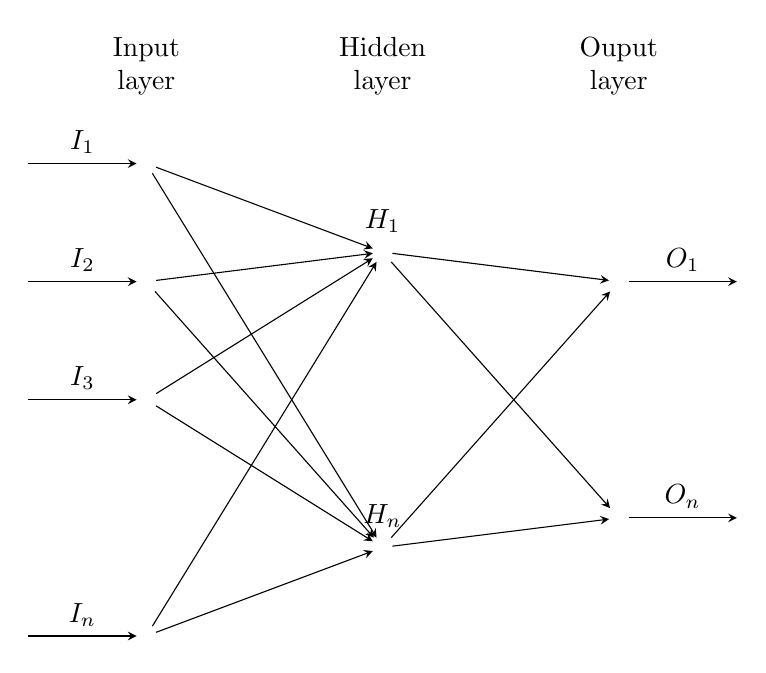
\begin{tikzpicture}[x=1.5cm, y=1.5cm, >=stealth]

\foreach \m/\l [count=\y] in {1,2,3,missing,4}
  \node [every neuron/.try, neuron \m/.try] (input-\m) at (0,2.5-\y) {};

\foreach \m [count=\y] in {1,missing,2}
  \node [every neuron/.try, neuron \m/.try ] (hidden-\m) at (2,2-\y*1.25) {};

\foreach \m [count=\y] in {1,missing,2}
  \node [every neuron/.try, neuron \m/.try ] (output-\m) at (4,1.5-\y) {};

\foreach \l [count=\i] in {1,2,3,n}
  \draw [<-] (input-\i) -- ++(-1,0)
    node [above, midway] {$I_\l$};

\foreach \l [count=\i] in {1,n}
  \node [above] at (hidden-\i.north) {$H_\l$};

\foreach \l [count=\i] in {1,n}
  \draw [->] (output-\i) -- ++(1,0)
    node [above, midway] {$O_\l$};

\foreach \i in {1,...,4}
  \foreach \j in {1,...,2}
    \draw [->] (input-\i) -- (hidden-\j);

\foreach \i in {1,...,2}
  \foreach \j in {1,...,2}
    \draw [->] (hidden-\i) -- (output-\j);

\foreach \l [count=\x from 0] in {Input, Hidden, Ouput}
  \node [align=center, above] at (\x*2,2) {\l \\ layer};

\end{tikzpicture}


\subsection{Including Code}

\begin{lstlisting}[language=Python]
        def hello_world_python():
            print("Hello floating world!")
\end{lstlisting}

% using R
%\begin{lstlisting}[language=R]
%hello_world_R <- function() {
%  print("Hello floating world!")
%}
%\end{lstlisting}

% using bash
%\begin{lstlisting}[language=bash]
%hello_world_bash() {
%  echo "Hello floating world!"
%}
%\end{lstlisting}

% using MATLAB
%\begin{lstlisting}[language=Matlab]
%function hello_world_matlab()
%  disp('Hello floating world!');
%end
%\end{lstlisting}


\subsection{Including Chemistry}

\begin{center}
	\chemfig{*6((=O)-N(-H)-(*5(-N=-N(-H)-))=-(=O)-N(-H)-)}
\end{center}

\subsection{Including Circuits} \nopagebreak

\begin{figure}[!hb] % h means here. t: top, b: bottom 
  \begin{center}
    \begin{circuitikz}
      \draw (0,0)
      to[V,v=$U_q$] (0,2) % The voltage source
      to[short] (2,2)
      to[R=$R_1$] (2,0) % The resistor
      to[short] (0,0);
    \end{circuitikz}
    \caption{Circuit 1.}
  \end{center}
\end{figure}

\FloatBarrier

\newpage
\thispagestyle{empty}
\section{Including an Article}

\includepdfset{pagecommand=\thispagestyle{scrheadings}} % adds page numbers to imported pdfs
\includepdf[pages=1-3, pagecommand={\pagestyle{empty}}]{pdfs/curie_notes.pdf}



%% === BACKMATER ====
% Unnumbered final parts (Conclusion, bibliography...)

\backmatter

%% === CONCLUSION ====
\chapter{Conclusion}

%% === BIBLIOGRAPHY ====
\bibliographystyle{plain}
\bibliography{biblio}
\nocite{hubel1962receptive}% adds uncited references to the bibliography

%% === LIST OF OPEN SOURCE RESOURCES ====
% to add 

%% === APPENDICES ====
\appendix

\chapter{Appendix 1}

\kant[1]

\chapter{Appendix 2}

%% === INDEX ====
\printindex % Prints the index
%\addcontentsline{toc}{chapter}{List of Abbreviations and Symbols}

\end{document}
